% Compile with: pdflatex -shell-escape tac_rules.tex
\documentclass[aspectratio=169]{beamer}
\usetheme{metropolis}
\metroset{block=fill}

%% ── Packages ──────────────────────────────────────────────────────────────
\usepackage{tikz}
\usetikzlibrary{arrows.meta, positioning, shapes.misc}
\usepackage{minted}
\usepackage{mathpartir}
\usepackage{amsmath}
\usepackage{booktabs}
\usepackage{xcolor}

%% ── Colours ───────────────────────────────────────────────────────────────
\definecolor{clrArt}{HTML}{AED6F1}    % artifact fill   (light blue)
\definecolor{clrArtBd}{HTML}{1F618D}  % artifact border (dark blue)
\definecolor{clrStg}{HTML}{FAD7A0}    % stage fill      (light amber)
\definecolor{clrStgBd}{HTML}{AF601A}  % stage border    (dark amber)

%% ── Notation shorthands ───────────────────────────────────────────────────
\newcommand{\trExpr}[1]{\mathit{trExpr}(#1)}
\newcommand{\trStmt}[1]{\mathit{trStmt}(#1)}
\newcommand{\trCond}[2]{\mathit{trCond}(#1,\;#2)}
\newcommand{\cat}{\mathbin{+\!\!+}}

%% Placeholder: mathpartir's \inferrule conflicts with beamer fragile frames
%% when conclusions contain \begin{array}+\\ — disable rules for now.
\AtBeginDocument{%
  \renewcommand{\inferrule}[3][]{%
    \vcenter{\hbox{$\scriptstyle[\text{Rule\ifx#1\empty\else{}: \textsc{#1}\fi}]$}}%
  }%
}

%% ── Meta ──────────────────────────────────────────────────────────────────
\title{MiniC Compiler}
\subtitle{From Annotated AST to Three Address Code}
\author{}
\date{\today}

\begin{document}

\maketitle

%% ══════════════════════════════════════════════════════════════════════════
%% Slide 1 – Compiler Pipeline
%% ══════════════════════════════════════════════════════════════════════════
\begin{frame}[shrink=5]{Compiler Pipeline}
\centering
\resizebox{0.98\textwidth}{!}{%
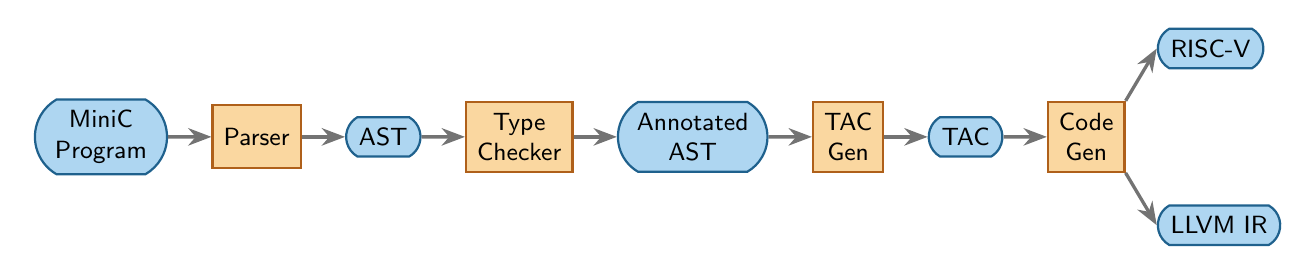
\begin{tikzpicture}[
  art/.style = {
    rounded rectangle,
    rounded rectangle arc length=120,
    draw=clrArtBd, fill=clrArt, line width=0.8pt,
    font=\sffamily\small, inner sep=4pt, align=center
  },
  stg/.style = {
    rectangle,
    draw=clrStgBd, fill=clrStg, line width=0.8pt,
    font=\sffamily\small, inner sep=4pt, align=center,
    minimum height=0.8cm
  },
  arr/.style  = {-Stealth, line width=1.2pt, color=black!55},
  node distance = 0.55cm
]
  \node[art]                            (minic)   {MiniC\\Program};
  \node[stg, right=of minic]            (parser)  {Parser};
  \node[art, right=of parser]           (ast)     {AST};
  \node[stg, right=of ast]              (tc)      {Type\\Checker};
  \node[art, right=of tc]               (aast)    {Annotated\\AST};
  \node[stg, right=of aast]             (tacgen)  {TAC\\Gen};
  \node[art, right=of tacgen]           (tac)     {TAC};
  \node[stg, right=of tac]              (codegen) {Code\\Gen};
  \node[art, above right=0.4cm and 0.55cm of codegen] (riscv) {RISC-V};
  \node[art, below right=0.4cm and 0.55cm of codegen] (llvm)  {LLVM IR};

  \draw[arr] (minic)              -- (parser);
  \draw[arr] (parser)             -- (ast);
  \draw[arr] (ast)                -- (tc);
  \draw[arr] (tc)                 -- (aast);
  \draw[arr] (aast)               -- (tacgen);
  \draw[arr] (tacgen)             -- (tac);
  \draw[arr] (tac)                -- (codegen);
  \draw[arr] (codegen.north east) -- (riscv.west);
  \draw[arr] (codegen.south east) -- (llvm.west);
\end{tikzpicture}%
}

\vspace{0.2em}
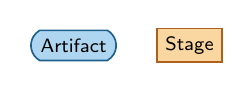
\begin{tikzpicture}[baseline, node distance=0.5cm]
  \node[rounded rectangle, rounded rectangle arc length=120,
        draw=clrArtBd, fill=clrArt, line width=0.6pt,
        font=\sffamily\scriptsize, inner sep=3pt] (a) {Artifact};
  \node[rectangle, draw=clrStgBd, fill=clrStg, line width=0.6pt,
        font=\sffamily\scriptsize, inner sep=3pt, right=0.5cm of a] {Stage};
\end{tikzpicture}
\end{frame}

%% ══════════════════════════════════════════════════════════════════════════
%% Slide 2 – What is Three Address Code?
%% ══════════════════════════════════════════════════════════════════════════
\begin{frame}[shrink=20]{Three Address Code}
  \begin{block}{Definition}
    An intermediate representation in which each instruction involves
    \textbf{at most three addresses}: a result and up to two operands.
    Intermediate values are made explicit through fresh \emph{temporaries}.
  \end{block}

  \smallskip
  \textbf{Instruction forms used in MiniC:}
  \begin{center}
    \footnotesize
    \begin{tabular}{lll}
      \toprule
      \textbf{Form}                  & \textbf{Syntax}                               & \textbf{Semantics}              \\
      \midrule
      Copy assignment                & \texttt{x := y}                               & $x \leftarrow y$                \\
      Binary assignment              & \texttt{t := a + b}                           & $t \leftarrow a \oplus b$       \\
      Cond.\ jump (relational)       & \texttt{if a >= b goto L}                     & jump if $a \geq b$              \\
      Cond.\ jump (boolean, false)   & \texttt{if\_false a goto L}                   & jump if $a$ is false            \\
      Cond.\ jump (boolean, true)    & \texttt{if a goto L}                          & jump if $a$ is true             \\
      Unconditional jump             & \texttt{goto L}                               & always jump to $L$              \\
      Label                          & \texttt{L:}                                   & marks a jump target             \\
      \bottomrule
    \end{tabular}
  \end{center}

  \smallskip
  \textbf{Addresses} are one of: a variable name, a constant literal,
  or a fresh temporary (\texttt{t1}, \texttt{t2}, \ldots).
\end{frame}

%% ══════════════════════════════════════════════════════════════════════════
%% Slide 3 – Assignment
%% ══════════════════════════════════════════════════════════════════════════
\begin{frame}[fragile]{Translation Rule: Assignment}
  \begin{columns}[T]
    \begin{column}{0.50\textwidth}
      \begin{block}{Rule}
        \vspace{0.3em}
        \[
          \inferrule[Assign]
            { \trExpr{e} \Rightarrow (a,\ I) }
            { \trStmt{\texttt{x = e}} \Rightarrow I \cat [\,\texttt{x} := a\,] }
        \]
        \vspace{0.1em}
      \end{block}
      \smallskip
      Translate $e$ to address $a$ with side-effect instructions $I$,
      then append the copy $\texttt{x} := a$.
    \end{column}
    \begin{column}{0.46\textwidth}
      \begin{block}{Examples}
        \begin{minted}[fontsize=\scriptsize]{c}
x = y;       // simple copy
x = a + b;   // with expression
        \end{minted}
        \vspace{0.3em}
        \begin{minted}[fontsize=\scriptsize]{text}
x := y

t1 := a + b
x  := t1
        \end{minted}
      \end{block}
    \end{column}
  \end{columns}
\end{frame}

%% ══════════════════════════════════════════════════════════════════════════
%% Slide 4 – Arithmetic Addition
%% ══════════════════════════════════════════════════════════════════════════
\begin{frame}[fragile]{Translation Rule: Arithmetic Addition}
  \begin{columns}[T]
    \begin{column}{0.52\textwidth}
      \begin{block}{Rule}
        \vspace{0.3em}
        \footnotesize
        %% TODO: restore inferrule[Add] — \begin{array}+\\ in conclusion
        %% conflicts with mathpartir's \mpr@makelist inside beamer fragile frames
        \[ \inferrule[Add]
            { \trExpr{e_1} \Rightarrow (a_1,\ I_1) \and
              \trExpr{e_2} \Rightarrow (a_2,\ I_2) \and
              t\ \text{fresh} }
            { \trExpr{e_1 + e_2} \Rightarrow
              \bigl(t,\;I_1 \cat I_2 \cat [\,t := a_1 + a_2\,]\bigr) }
        \]
        \vspace{0.2em}
      \end{block}
      A fresh temporary $t$ holds the result.
      Sub-expressions are evaluated left-to-right.
    \end{column}
    \begin{column}{0.44\textwidth}
      \begin{block}{Simple}
        \begin{minted}[fontsize=\small]{c}
x = a + b;
        \end{minted}
        \begin{minted}[fontsize=\small]{text}
t1 := a + b
x  := t1
        \end{minted}
      \end{block}
      \begin{block}{Nested}
        \begin{minted}[fontsize=\small]{c}
x = (a + b) + c;
        \end{minted}
        \begin{minted}[fontsize=\small]{text}
t1 := a + b
t2 := t1 + c
x  := t2
        \end{minted}
      \end{block}
    \end{column}
  \end{columns}
\end{frame}

%% ══════════════════════════════════════════════════════════════════════════
%% Slide 5 – If-Then-Else
%% ══════════════════════════════════════════════════════════════════════════
\begin{frame}[fragile]{Translation Rule: If-Then-Else}
  \begin{columns}[T]
    \begin{column}{0.55\textwidth}
      \begin{block}{Rule}
        \vspace{0.3em}
        \scriptsize
        \[
          \inferrule[IfElse]
            {
              L_e,\ L_{\mathrm{end}}\ \text{fresh} \\
              \trCond{c}{L_e} \Rightarrow I_c \\
              \trStmt{s_1} \Rightarrow I_t \quad
              \trStmt{s_2} \Rightarrow I_f
            }
            {{
              \begin{array}{l}
                \trStmt{\texttt{if}\,(c)\;s_1\;\texttt{else}\;s_2}
                \;\Rightarrow \\
                \quad I_c \cat I_t \cat [\texttt{goto}\ L_{\mathrm{end}}] \\
                \quad\cat [L_e\texttt{:}] \cat I_f \cat [L_{\mathrm{end}}\texttt{:}]
              \end{array}
            }}
        \]
        \vspace{0.2em}
      \end{block}
      $\mathit{trCond}$ emits a jump to $L_e$ when $c$ is \textbf{false};
      the then-branch falls through on the true path.
    \end{column}
    \begin{column}{0.41\textwidth}
      \begin{block}{Example}
        \begin{minted}[fontsize=\scriptsize]{c}
if (x > 0) {
  y = 1;
} else {
  y = 0;
}
        \end{minted}
        \vspace{0.3em}
        \begin{minted}[fontsize=\scriptsize]{text}
if x <= 0 goto L1
y := 1
goto L2
L1:
y := 0
L2:
        \end{minted}
      \end{block}
    \end{column}
  \end{columns}
\end{frame}

%% ══════════════════════════════════════════════════════════════════════════
%% Slide 6 – Relational Operators
%% ══════════════════════════════════════════════════════════════════════════
\begin{frame}[fragile]{Translation Rule: Relational Operators}
  \begin{columns}[T]
    \begin{column}{0.50\textwidth}
      \begin{block}{Rule}
        \vspace{0.3em}
        \footnotesize
        \[
          \inferrule[Rel]
            {
              \trExpr{e_1} \Rightarrow (a_1,\ I_1) \\
              \trExpr{e_2} \Rightarrow (a_2,\ I_2)
            }
            {{
              \begin{array}{l}
                \trCond{e_1\ \mathit{op}\ e_2}{L_f} \;\Rightarrow \\
                \quad I_1 \cat I_2 \cat
                [\texttt{if}\ a_1\ \overline{\mathit{op}}\ a_2\ \texttt{goto}\ L_f]
              \end{array}
            }}
        \]
        \vspace{0.2em}
      \end{block}
      \begin{center}
        \small
        \begin{tabular}{cc}
          \toprule
          $\mathit{op}$ & $\overline{\mathit{op}}$ \\
          \midrule
          \texttt{<}  & \texttt{>=} \\
          \texttt{<=} & \texttt{>}  \\
          \texttt{>}  & \texttt{<=} \\
          \texttt{>=} & \texttt{<}  \\
          \texttt{==} & \texttt{!=} \\
          \texttt{!=} & \texttt{==} \\
          \bottomrule
        \end{tabular}
      \end{center}
    \end{column}
    \begin{column}{0.46\textwidth}
      \begin{block}{Example: \texttt{x < y}}
        \begin{minted}[fontsize=\small]{c}
if (x < y) { ... }
        \end{minted}
        \vspace{0.3em}
        \begin{minted}[fontsize=\small]{text}
; jump to Lf when x < y is FALSE
if x >= y goto Lf
        \end{minted}
      \end{block}
      \begin{alertblock}{Key Insight}
        We emit a jump to $L_f$ when the condition is \emph{false},
        so we use the \textbf{negated} operator.
        The fall-through path is the ``true'' branch.
      \end{alertblock}
    \end{column}
  \end{columns}
\end{frame}

%% ══════════════════════════════════════════════════════════════════════════
%% Slide 7 – trCond Base Cases
%% ══════════════════════════════════════════════════════════════════════════
\begin{frame}[fragile,shrink=5]{Translation Rule: \textit{trCond} Base Cases}
  \begin{columns}[T]
    \begin{column}{0.52\textwidth}
      \begin{block}{Rules}
        \vspace{0.3em}
        \footnotesize
        \[
          \inferrule[CondTrue]
            { }
            { \trCond{\texttt{true}}{L_f} \;\Rightarrow\; [] }
        \]
        \[
          \inferrule[CondFalse]
            { }
            { \trCond{\texttt{false}}{L_f} \;\Rightarrow\; [\,\texttt{goto}\ L_f\,] }
        \]
        \[
          \inferrule[CondIdent]
            { }
            {{
              \begin{array}{l}
                \trCond{x}{L_f} \;\Rightarrow \\
                \quad[\,\texttt{if\_false}\ x\ \texttt{goto}\ L_f\,]
              \end{array}
            }}
        \]
        \vspace{0.2em}
      \end{block}
      \texttt{true} always falls through; \texttt{false} always jumps;
      a boolean identifier jumps only when it is false.
    \end{column}
    \begin{column}{0.44\textwidth}
      \begin{block}{Boolean variable condition}
        \begin{minted}[fontsize=\footnotesize]{c}
if (flag) { ... }
        \end{minted}
        \vspace{0.3em}
        \begin{minted}[fontsize=\footnotesize]{text}
if_false flag goto Lf
; fall-through: flag is true
        \end{minted}
      \end{block}
      \begin{block}{Literal conditions}
        \begin{minted}[fontsize=\footnotesize]{text}
; trCond(true,  Lf) => (nothing)
; trCond(false, Lf) => goto Lf
        \end{minted}
      \end{block}
    \end{column}
  \end{columns}
\end{frame}

%% ══════════════════════════════════════════════════════════════════════════
%% Slide 8 – Short-Circuit AND (trCond)
%% ══════════════════════════════════════════════════════════════════════════
\begin{frame}[fragile]{Translation Rule: \texttt{\&\&} (Short-Circuit AND) — \textit{trCond}}
  \begin{columns}[T]
    \begin{column}{0.50\textwidth}
      \begin{block}{Rule}
        \vspace{0.3em}
        \[
          \inferrule[And]
            {
              \trCond{e_1}{L_f} \Rightarrow I_1 \\
              \trCond{e_2}{L_f} \Rightarrow I_2
            }
            {
              \trCond{e_1 \mathbin{\texttt{\&\&}} e_2}{L_f}
              \;\Rightarrow\; I_1 \cat I_2
            }
        \]
        \vspace{0.1em}
      \end{block}
      \smallskip
      If $e_1$ is \textbf{false} the jump to $L_f$ fires immediately
      — $e_2$ is \textbf{never evaluated}.
    \end{column}
    \begin{column}{0.46\textwidth}
      \begin{block}{Example}
        \begin{minted}[fontsize=\small]{c}
if (x > 0 && y < 10) {
  ...
}
        \end{minted}
        \vspace{0.3em}
        \begin{minted}[fontsize=\small]{text}
if x <= 0  goto Lf
if y >= 10 goto Lf
; fall-through: both true
        \end{minted}
      \end{block}
    \end{column}
  \end{columns}
\end{frame}

%% ══════════════════════════════════════════════════════════════════════════
%% Slide 9 – Short-Circuit OR (trCond)
%% ══════════════════════════════════════════════════════════════════════════
\begin{frame}[fragile]{Translation Rule: \texttt{||} (Short-Circuit OR) — \textit{trCond}}
  \begin{columns}[T]
    \begin{column}{0.55\textwidth}
      \begin{block}{Rule}
        \vspace{0.3em}
        \scriptsize
        \[
          \inferrule[Or]
            {
              L_{\mathrm{skip}}\ \text{fresh} \\
              \trExpr{e_1} \Rightarrow (a_1,\ I_1) \\
              \trCond{e_2}{L_f} \Rightarrow I_2
            }
            {{
              \begin{array}{l}
                \trCond{e_1 \mathbin{\texttt{||}} e_2}{L_f} \;\Rightarrow \\
                \quad I_1 \cat [\texttt{if}\ a_1\ \texttt{goto}\ L_{\mathrm{skip}}] \\
                \quad\cat I_2 \cat [L_{\mathrm{skip}}\texttt{:}]
              \end{array}
            }}
        \]
        \vspace{0.2em}
      \end{block}
      If $e_1$ is \textbf{true}, we jump over $e_2$ entirely
      — it is \textbf{never evaluated} (short-circuit).
    \end{column}
    \begin{column}{0.41\textwidth}
      \begin{block}{Example}
        \begin{minted}[fontsize=\scriptsize]{c}
if (found || count < 10) {
  ...
}
        \end{minted}
        \vspace{0.3em}
        \begin{minted}[fontsize=\scriptsize]{text}
if found goto Lskip
if count >= 10 goto Lf
Lskip:
; fall-through: at least one true
        \end{minted}
      \end{block}
    \end{column}
  \end{columns}
\end{frame}

%% ══════════════════════════════════════════════════════════════════════════
%% Slide 10 – Logical NOT (trCond)
%% ══════════════════════════════════════════════════════════════════════════
\begin{frame}[fragile]{Translation Rule: \texttt{!} (Logical NOT) — \textit{trCond}}
  \begin{columns}[T]
    \begin{column}{0.50\textwidth}
      \begin{block}{Rule}
        \vspace{0.5em}
        \[
          \inferrule[Not]
            { \trExpr{e} \Rightarrow (a,\ I) }
            {
              \trCond{\texttt{!}e}{L_f}
              \;\Rightarrow\;
              I \cat [\texttt{if}\ a\ \texttt{goto}\ L_f]
            }
        \]
        \vspace{0.3em}
      \end{block}
      \medskip
      $\texttt{!}e$ is false exactly when $e$ is \textbf{true}.
      We therefore jump to $L_f$ when $a$ holds a truthy value.
    \end{column}
    \begin{column}{0.46\textwidth}
      \begin{block}{Example}
        \begin{minted}[fontsize=\small]{c}
if (!flag) {
  ...
}
        \end{minted}
        \vspace{0.3em}
        \begin{minted}[fontsize=\small]{text}
; trCond(!flag, Lf)
if flag goto Lf
; fall-through: flag was false
        \end{minted}
      \end{block}
    \end{column}
  \end{columns}
\end{frame}

%% ══════════════════════════════════════════════════════════════════════════
%% Slide 11 – trExpr vs trCond for Booleans
%% ══════════════════════════════════════════════════════════════════════════
\begin{frame}{Boolean Expressions: Two Translation Contexts}
  \begin{block}{\textit{trCond} — boolean drives control flow}
    Used when the boolean is the condition of an \texttt{if} or \texttt{while}.
    The result is expressed as \emph{conditional jumps}; no temporary is needed.
    \begin{itemize}
      \item \texttt{if (a \&\& b) \{\ldots\}} $\;\to\;$ two conditional jumps, no temp
    \end{itemize}
  \end{block}

  \vspace{0.4em}

  \begin{block}{\textit{trExpr} — boolean stored as a value}
    Used when the boolean result must be \emph{assigned to a variable}.
    The result is \emph{materialised} into a fresh temporary via labelled code.
    \begin{itemize}
      \item \texttt{x = a \&\& b;} $\;\to\;$ labels, conditional jumps, \texttt{t := true/false}, copy
    \end{itemize}
  \end{block}

  \vspace{0.4em}
  The following three slides show the \textit{trExpr} rules for
  \texttt{!}, \texttt{\&\&}, and \texttt{||}.
\end{frame}

%% ══════════════════════════════════════════════════════════════════════════
%% Slide 12 – trExpr: Logical NOT
%% ══════════════════════════════════════════════════════════════════════════
\begin{frame}[fragile]{Translation Rule: \texttt{trExpr} — Logical NOT}
  \begin{columns}[T]
    \begin{column}{0.56\textwidth}
      \begin{block}{Rule}
        \vspace{0.3em}
        \scriptsize
        \[
          \inferrule[NotExpr]
            {
              \trExpr{e} \Rightarrow (a,\ I) \\
              t,\ L_f,\ L_e\ \text{fresh}
            }
            {{
              \begin{array}{l}
                \trExpr{\texttt{!}e} \;\Rightarrow\; \bigl(t,\; I \\
                \cat [\texttt{if\_false}\ a\ \texttt{goto}\ L_f] \\
                \cat [\,t := \texttt{false},\;\texttt{goto}\ L_e\,] \\
                \cat [\,L_f\texttt{:},\;t := \texttt{true},\;L_e\texttt{:}\,]\bigr)
              \end{array}
            }}
        \]
        \vspace{0.2em}
      \end{block}
      \smallskip
      Fall-through ($a$ true) $\Rightarrow$ $t$ gets \texttt{false}.\\
      Jump to $L_f$ ($a$ false) $\Rightarrow$ $t$ gets \texttt{true}.
    \end{column}
    \begin{column}{0.40\textwidth}
      \begin{block}{Example: \texttt{x = !flag}}
        \begin{minted}[fontsize=\scriptsize]{c}
x = !flag;
        \end{minted}
        \vspace{0.3em}
        \begin{minted}[fontsize=\scriptsize]{text}
if_false flag goto L1
t1 := false
goto L2
L1:
t1 := true
L2:
x := t1
        \end{minted}
      \end{block}
    \end{column}
  \end{columns}
\end{frame}

%% ══════════════════════════════════════════════════════════════════════════
%% Slide 13 – trExpr: Logical AND
%% ══════════════════════════════════════════════════════════════════════════
\begin{frame}[fragile]{Translation Rule: \texttt{trExpr} — Logical AND}
  \begin{columns}[T]
    \begin{column}{0.56\textwidth}
      \begin{block}{Rule}
        \vspace{0.3em}
        \scriptsize
        \[
          \inferrule[AndExpr]
            {
              \trExpr{e_1} \Rightarrow (a_1,\ I_1) \\
              \trExpr{e_2} \Rightarrow (a_2,\ I_2) \\
              t,\ L_f,\ L_e\ \text{fresh}
            }
            {{
              \begin{array}{l}
                \trExpr{e_1 \mathbin{\texttt{\&\&}} e_2} \;\Rightarrow\; \bigl(t,\; I_1 \\
                \cat [\texttt{if\_false}\ a_1\ \texttt{goto}\ L_f] \\
                \cat\; I_2 \cat [\texttt{if\_false}\ a_2\ \texttt{goto}\ L_f] \\
                \cat [\,t := \texttt{true},\;\texttt{goto}\ L_e\,] \\
                \cat [\,L_f\texttt{:},\;t := \texttt{false},\;L_e\texttt{:}\,]\bigr)
              \end{array}
            }}
        \]
        \vspace{0.1em}
      \end{block}
      \smallskip
      $e_2$ is \textbf{not evaluated} when $e_1$ is false (short-circuit).
    \end{column}
    \begin{column}{0.40\textwidth}
      \begin{block}{Example: \texttt{x = a \&\& b}}
        \begin{minted}[fontsize=\scriptsize]{c}
x = a && b;
        \end{minted}
        \vspace{0.3em}
        \begin{minted}[fontsize=\scriptsize]{text}
if_false a goto L1
if_false b goto L1
t1 := true
goto L2
L1:
t1 := false
L2:
x := t1
        \end{minted}
      \end{block}
    \end{column}
  \end{columns}
\end{frame}

%% ══════════════════════════════════════════════════════════════════════════
%% Slide 14 – trExpr: Logical OR
%% ══════════════════════════════════════════════════════════════════════════
\begin{frame}[fragile]{Translation Rule: \texttt{trExpr} — Logical OR}
  \begin{columns}[T]
    \begin{column}{0.56\textwidth}
      \begin{block}{Rule}
        \vspace{0.3em}
        \scriptsize
        \[
          \inferrule[OrExpr]
            {
              \trExpr{e_1} \Rightarrow (a_1,\ I_1) \\
              \trExpr{e_2} \Rightarrow (a_2,\ I_2) \\
              t,\ L_t,\ L_f,\ L_e\ \text{fresh}
            }
            {{
              \begin{array}{l}
                \trExpr{e_1 \mathbin{\texttt{||}} e_2} \;\Rightarrow\; \bigl(t,\; I_1 \\
                \cat [\texttt{if\_false}\ a_1\ \texttt{goto}\ L_f,\;\texttt{goto}\ L_t] \\
                \cat [\,L_f\texttt{:}\,] \cat\; I_2 \\
                \cat [\texttt{if}\ a_2\ \texttt{goto}\ L_t] \\
                \cat [\,t := \texttt{false},\;\texttt{goto}\ L_e\,] \\
                \cat [\,L_t\texttt{:},\;t := \texttt{true},\;L_e\texttt{:}\,]\bigr)
              \end{array}
            }}
        \]
        \vspace{0.1em}
      \end{block}
      \smallskip
      $e_2$ is \textbf{not evaluated} when $e_1$ is true (short-circuit).
    \end{column}
    \begin{column}{0.40\textwidth}
      \begin{block}{Example: \texttt{x = a || b}}
        \begin{minted}[fontsize=\scriptsize]{c}
x = a || b;
        \end{minted}
        \vspace{0.3em}
        \begin{minted}[fontsize=\scriptsize]{text}
if_false a goto L2
goto L1
L2:
if b goto L1
t1 := false
goto L3
L1:
t1 := true
L3:
x := t1
        \end{minted}
      \end{block}
    \end{column}
  \end{columns}
\end{frame}

\end{document}
